\documentclass[9pt]{beamer}

\usetheme{TUDo}



% Encoding je nach Compiler
\ifluatex
\usepackage[utf8]{luainputenc}
\else
\usepackage[utf8]{inputenc}
\usepackage[T1]{fontenc}
\fi

%Links
\usepackage[]{hyperref}

%Float
\usepackage[]{float}

%Alternative texts for images (and other)
\usepackage[]{pdfcomment}

\renewcommand{\figurename}{Fig.}

%%%%%%%%%%%%%%%%%%%%%%%%%%%%%%%%%%%%%%%%%%%%%%%%%%%%%%%%%%%%%%%%%%%%%%%%%%%%%%%%
%%%%%-------------Hier Titel/Autor/Grafik/Lehrstuhl eintragen--------------%%%%%
%%%%%%%%%%%%%%%%%%%%%%%%%%%%%%%%%%%%%%%%%%%%%%%%%%%%%%%%%%%%%%%%%%%%%%%%%%%%%%%%

\title{Accessmail - an accessible E-Mail Client}
\author{Simon Demming, Jonas Langenberg}
\institute[]{\par\smallskip\smallskip Faculty for Rehabilitation Sciences\\ Faculty for Computer Science}


\begin{document}

	\begin{frame}
		\setcounter{framenumber}{0}
	    \titlepage
	\end{frame}
	
	\begin{frame}
		\begin{columns}[T]
        		\begin{column}{0.49\textwidth}
        			\begin{figure}
        				\centering
        				\pdftooltip{\includegraphics[scale=0.1]{Images/jonas.png}}{A picture of Jonas Langenberg}
        			\end{figure}
        		\end{column}
        		\begin{column}{0.49\textwidth}
		    		\begin{itemize}
			    		\item Jonas Langenberg
			    		\item 23 years
			    		\item 7th semester BA Computer Science
          		\end{itemize}
        		\end{column}
    		\end{columns}
	\end{frame}
	
	\begin{frame}
		\begin{columns}[T]
        		\begin{column}{0.49\textwidth}
        			\begin{figure}
        				\centering
        				\pdftooltip{\includegraphics[scale=0.2]{Images/simon.png}}{A picture of Simon Demming}
        			\end{figure}
        		\end{column}
        		\begin{column}{0.49\textwidth}
          		\begin{itemize}
              		\item Simon Demming
              		\item 22 years
              		\item 6th semester BA Computer Science
          		\end{itemize}
        		\end{column}
    		\end{columns}
	\end{frame}
	
	\section{Introduction}
		
		\begin{frame}
			\frametitle{Introduction}
			
			Email as a very important communication platform used for
			\begin{itemize}
				\item Private communication
				\item Labour affairs
				\item Finances
				\item Entertainment
			\end{itemize}
		\end{frame}
		
		\begin{frame}
			\frametitle{Typical German Provider}
			\begin{figure}
				\centering
				\pdftooltip{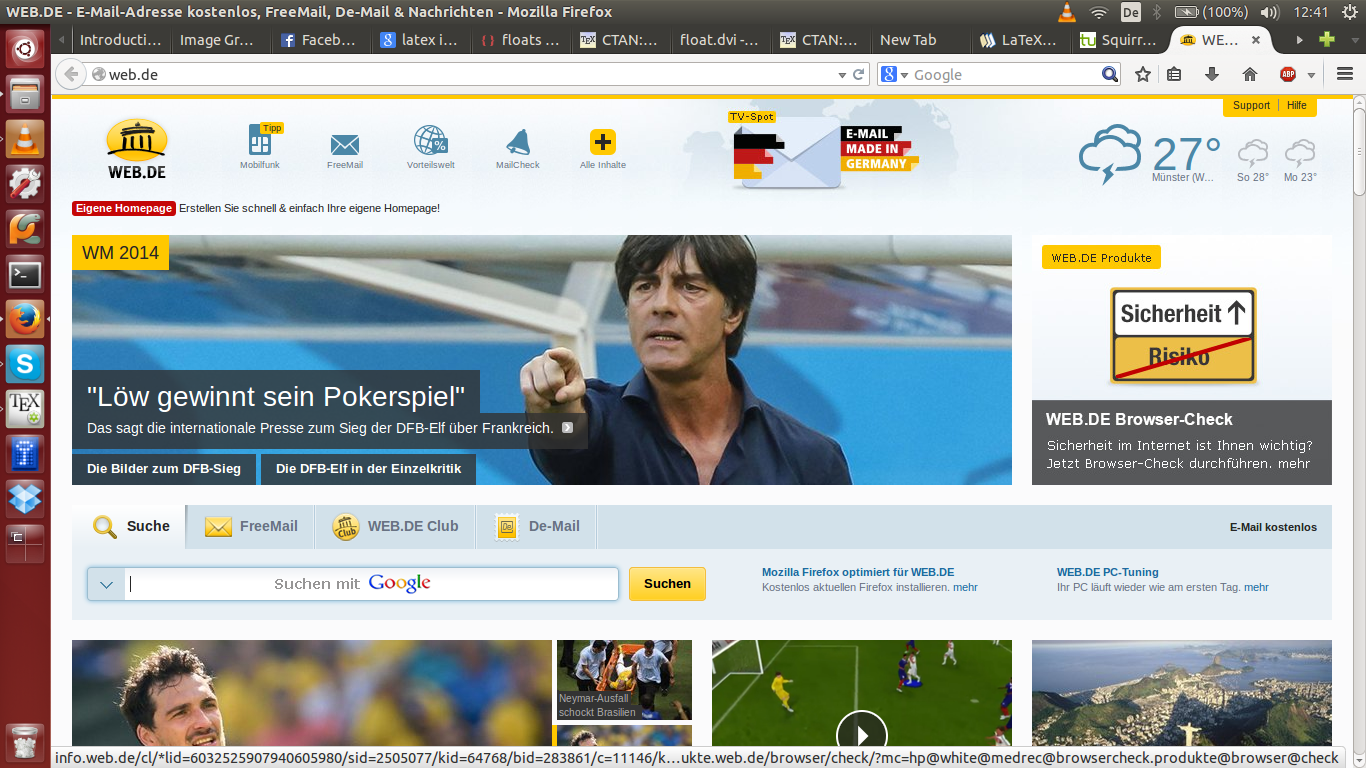
\includegraphics[scale=0.2]{Images/webstart.png}}{A picture of the web.de start page. You have no clear structure and the function we aim for is hard to find.}
			\end{figure}
		\end{frame}
		
		\begin{frame}
			\frametitle{Typical Scam}
			\begin{figure}
				\centering
				\pdftooltip{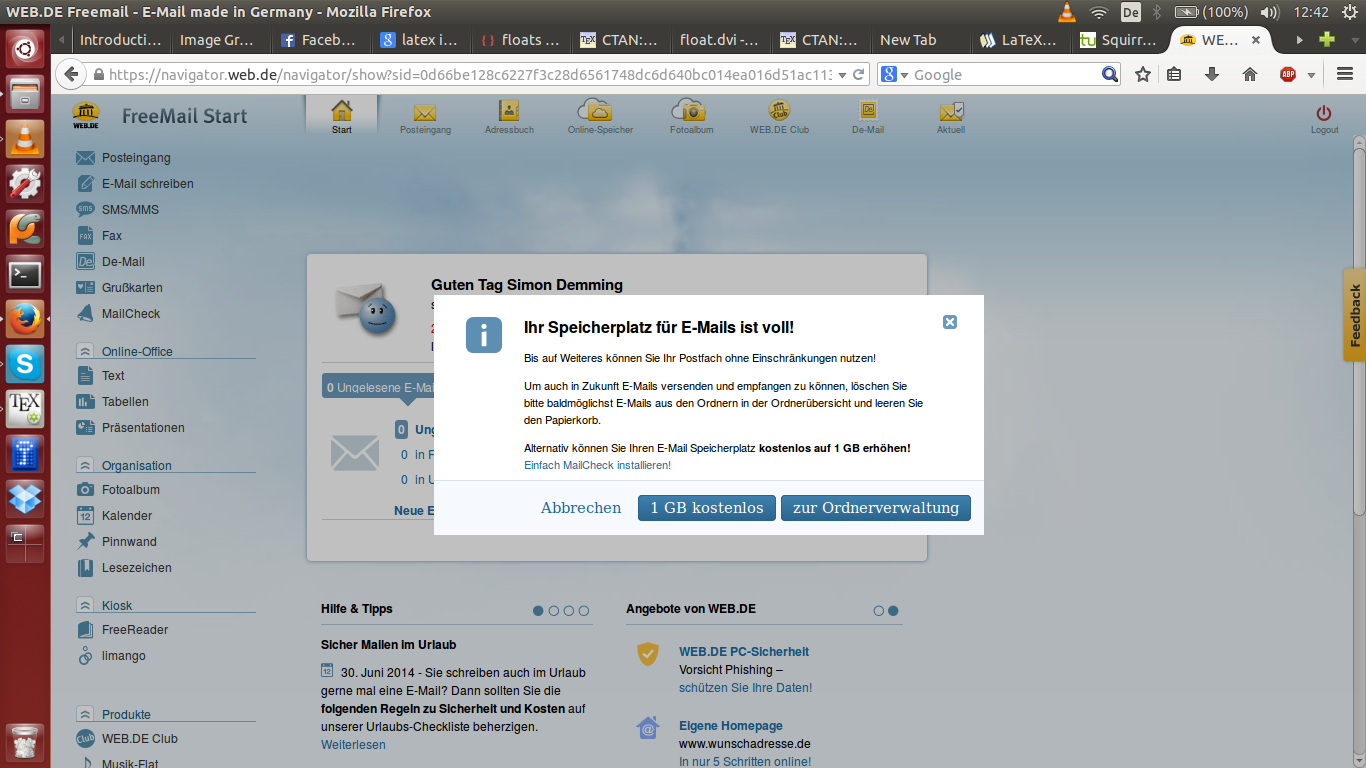
\includegraphics[scale=0.2]{Images/webstartmail.png}}{A picture of the web.de inbox. The inbox is too full. The provider tries to sell more web space for money.}
				
			\end{figure}
		\end{frame}
		
		\begin{frame}
			\frametitle{Error prone web application}
			\begin{figure}
				\centering
				\pdftooltip{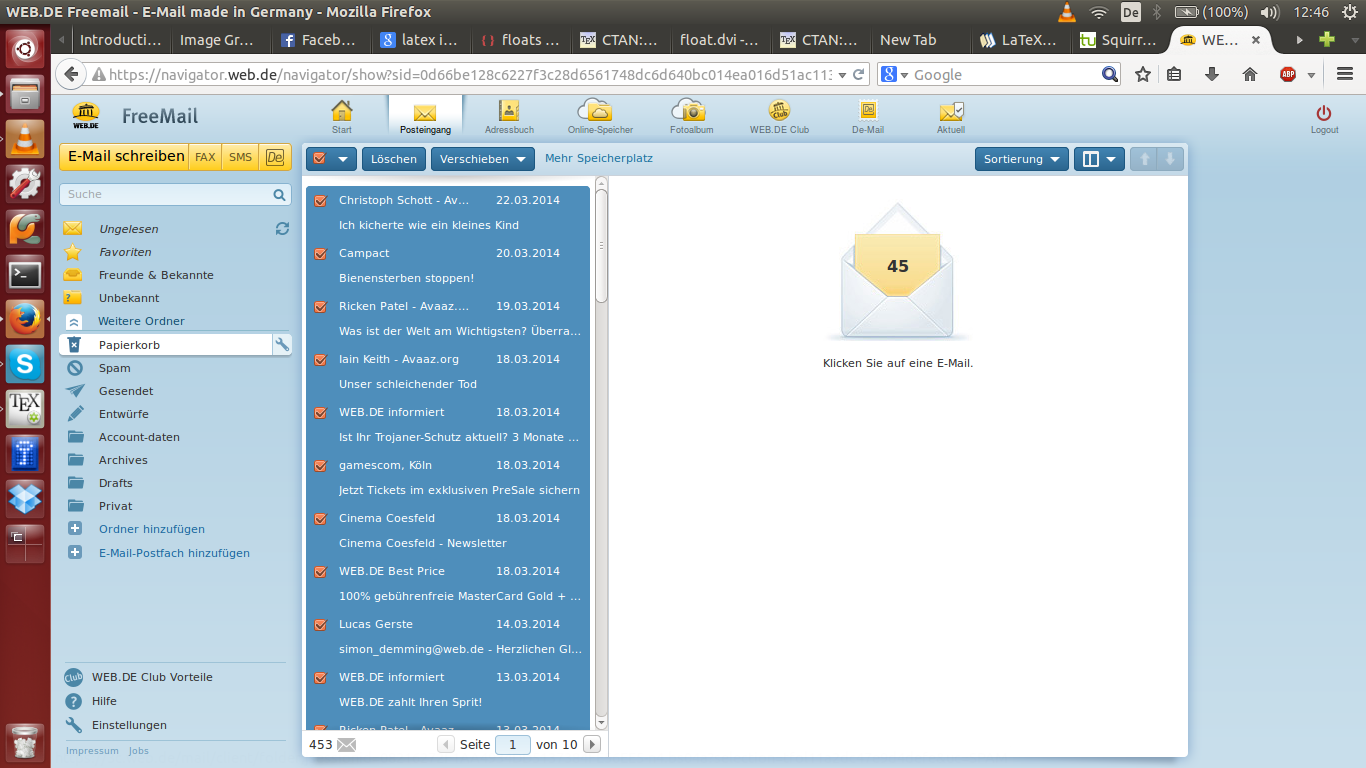
\includegraphics[scale=0.2]{Images/deletemailserror.png}}{A picture of the web.de trash box. The interface crashed when the user tried to delete emails.}
				
			\end{figure}
		\end{frame}
		
		\begin{frame}
			\frametitle{No standardization}
			\begin{figure}
				\centering
				\pdftooltip{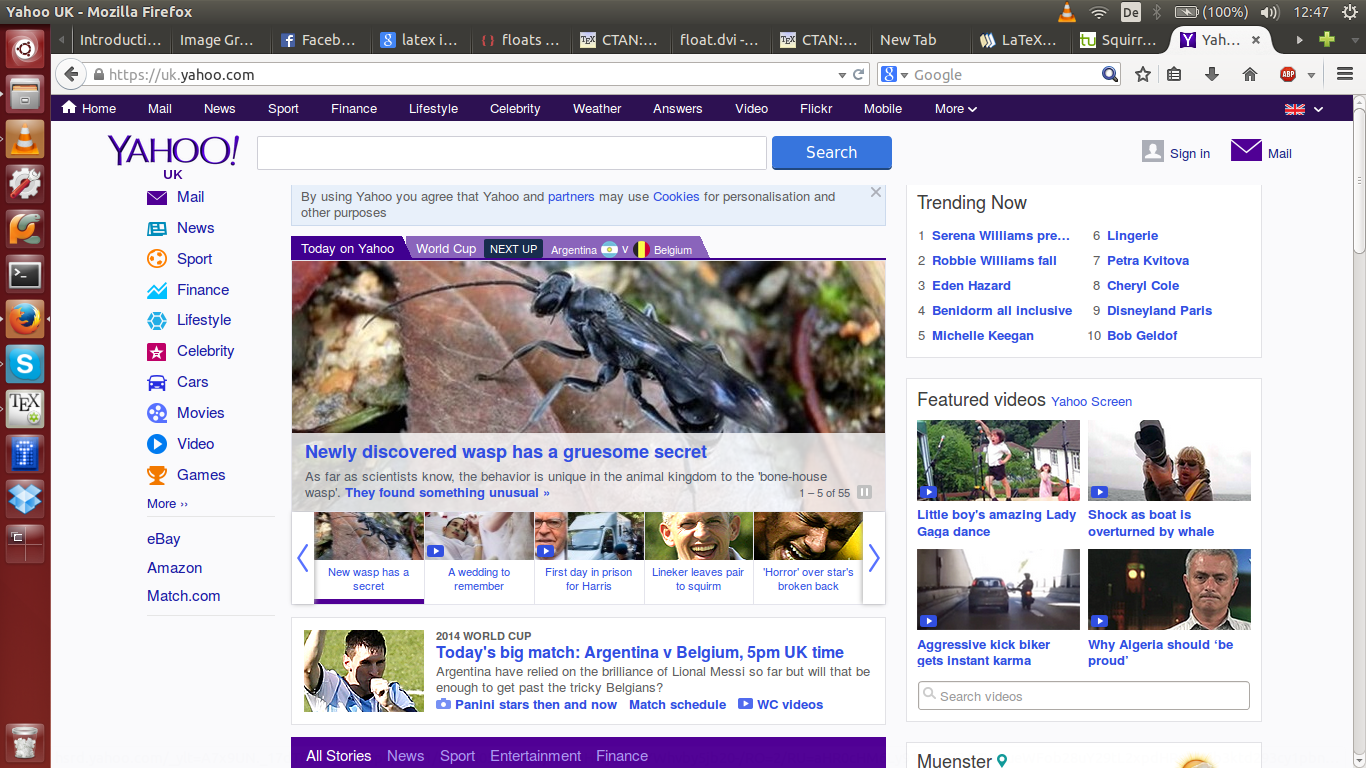
\includegraphics[scale=0.2]{Images/yahoostart.png}}{A picture of the yahoo.com start page. The layout is totally different from the web.de start page.}
			\end{figure}
		\end{frame}
		
		\begin{frame}
			\frametitle{Email is not easy!}
			Web applications of email providers:
			\begin{itemize}
				\item Are overloaded in functionality
				\item Try to rip you off
				\item Are technically complex
			\end{itemize}
		\end{frame}
		
		\begin{frame}
			\frametitle{Email is not easy!}
			\begin{figure}
				\centering
				\pdftooltip{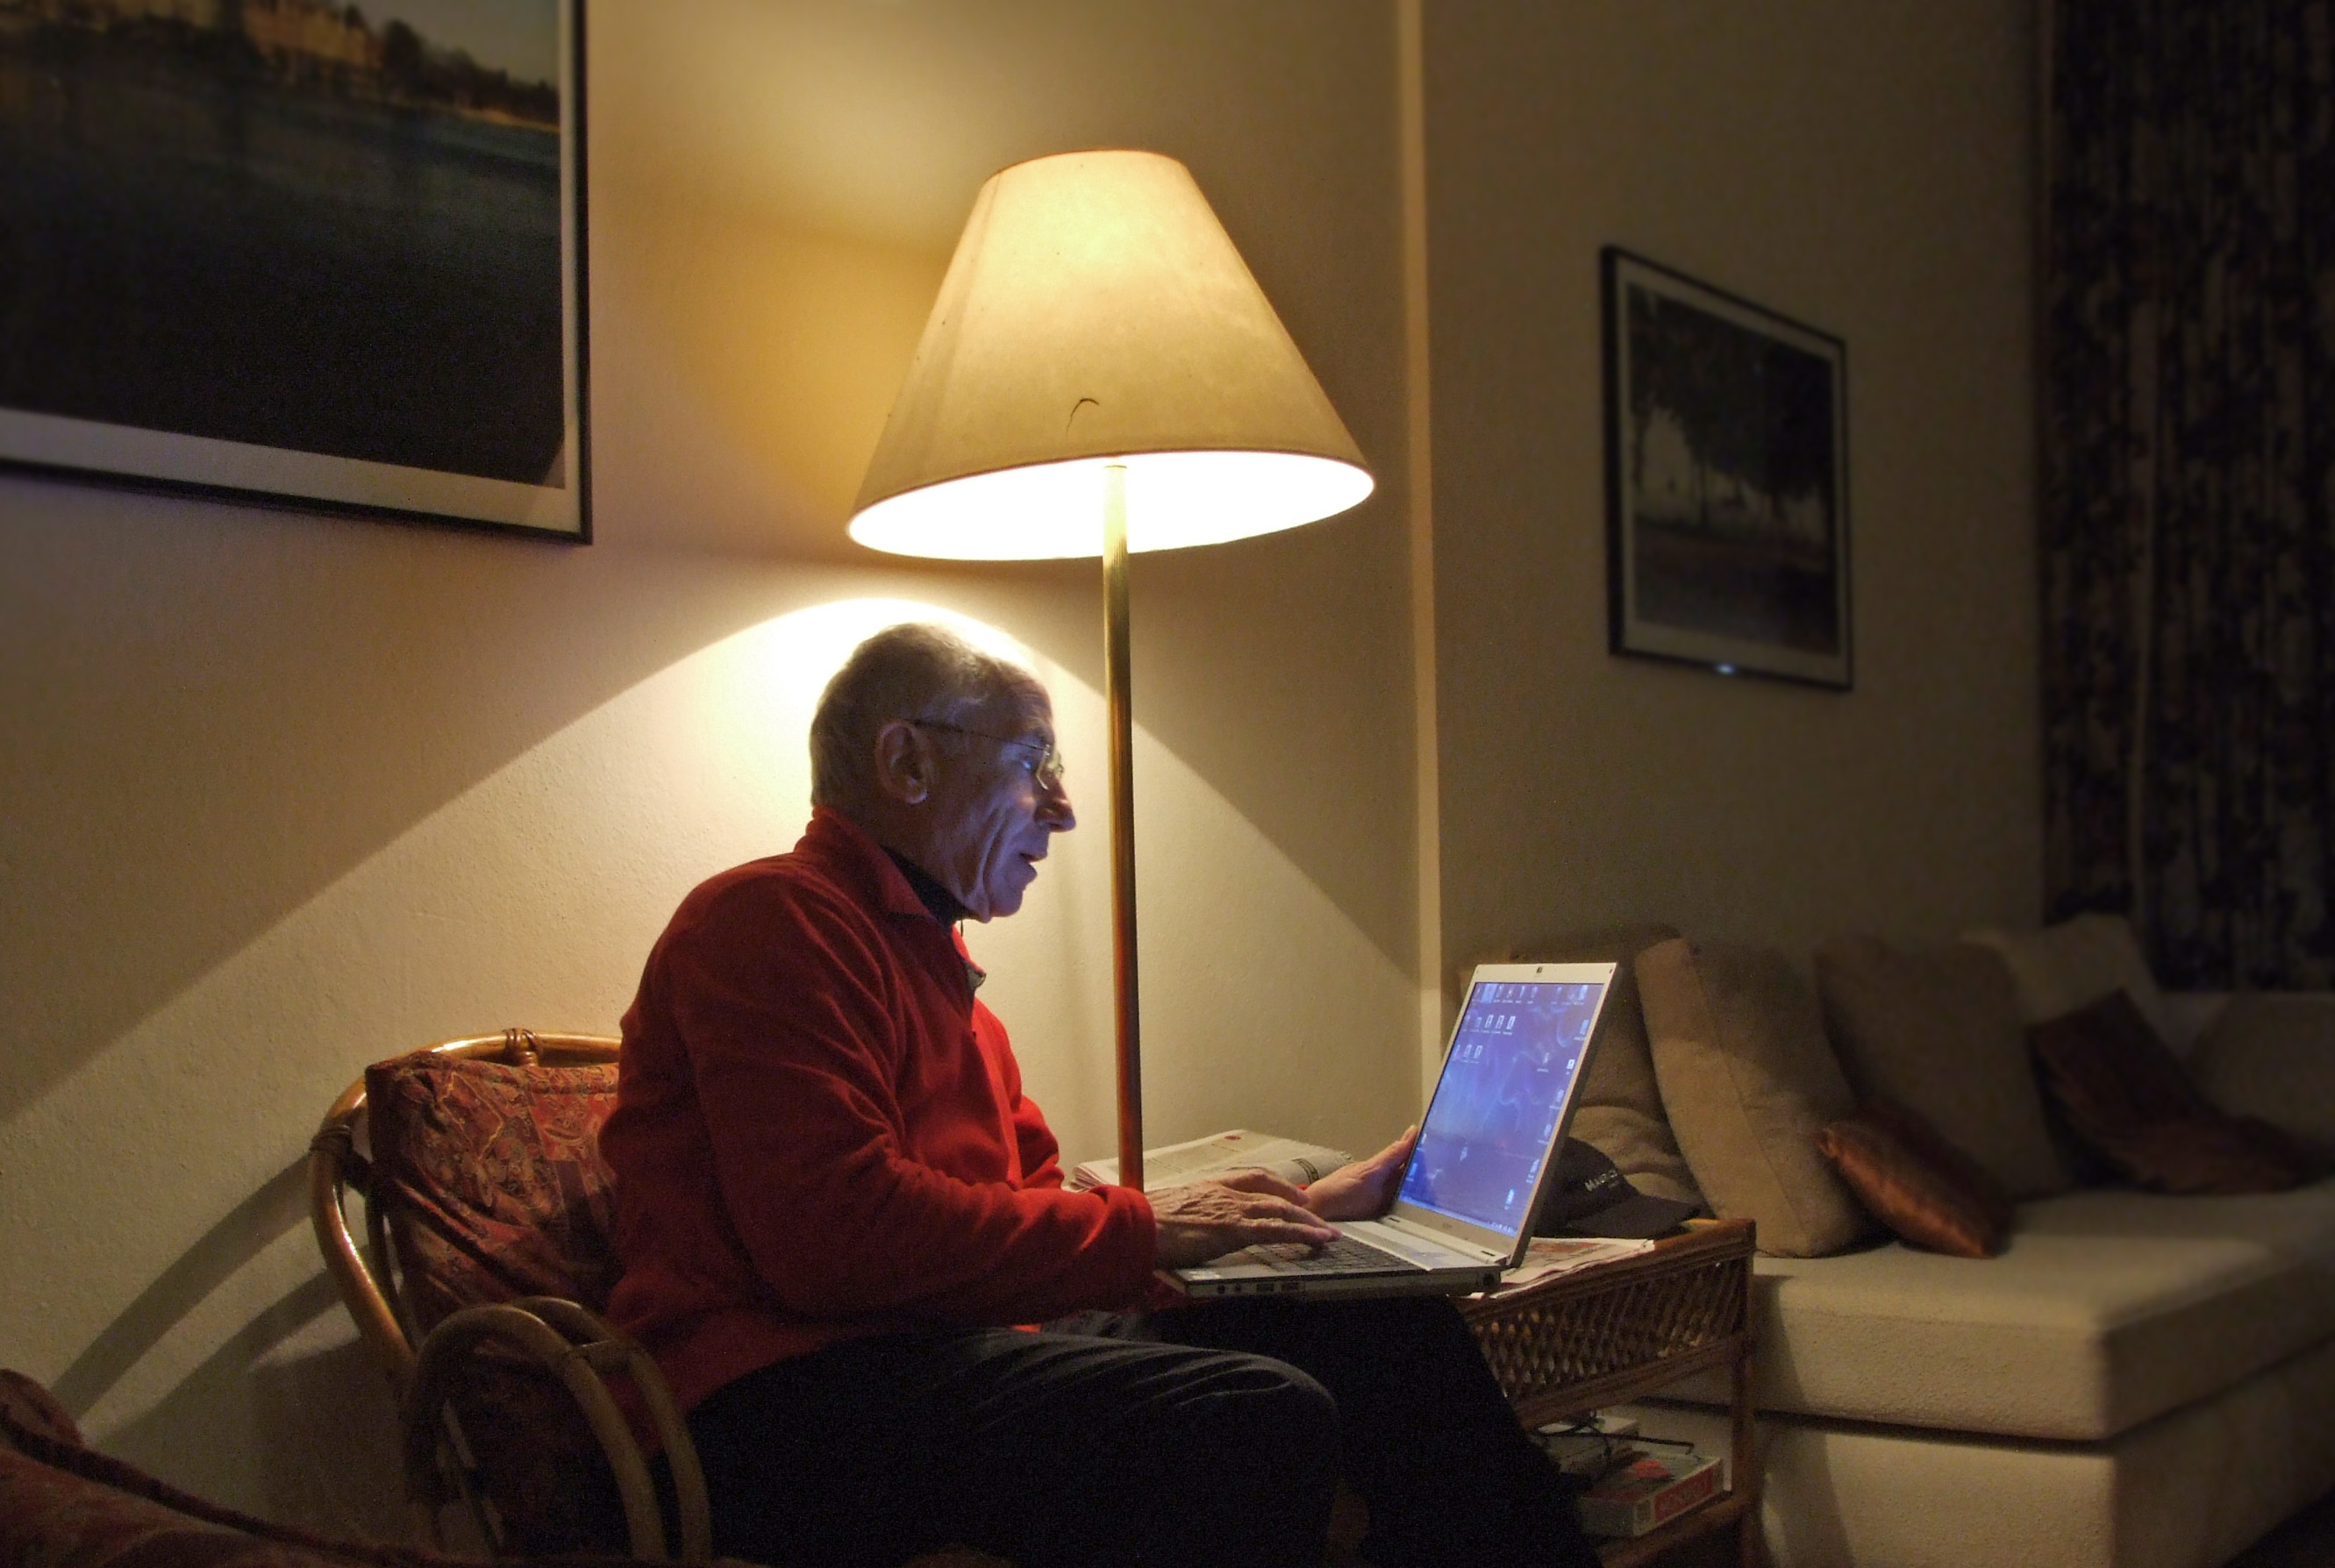
\includegraphics[scale=0.085]{Images/computersenior.jpg}}{A picture of an old man using a laptop.}
				\caption{Rainer Sturm  / pixelio.de}
			\end{figure}
		\end{frame}
		
		\begin{frame}
			\frametitle{Our Approach}
			We cannot offer a new provider.\\
			We cannot establish standards.\\
			But we can design an own front end.\\
			Design it to be universal.\\
			And verify it with an User Centered Design approach.
		\end{frame}
	
	\section{Our Approach}
		\subsection{Preparations}
		
		\begin{frame}
			\frametitle{Preparations}
			\begin{figure}
				\centering
				\pdftooltip{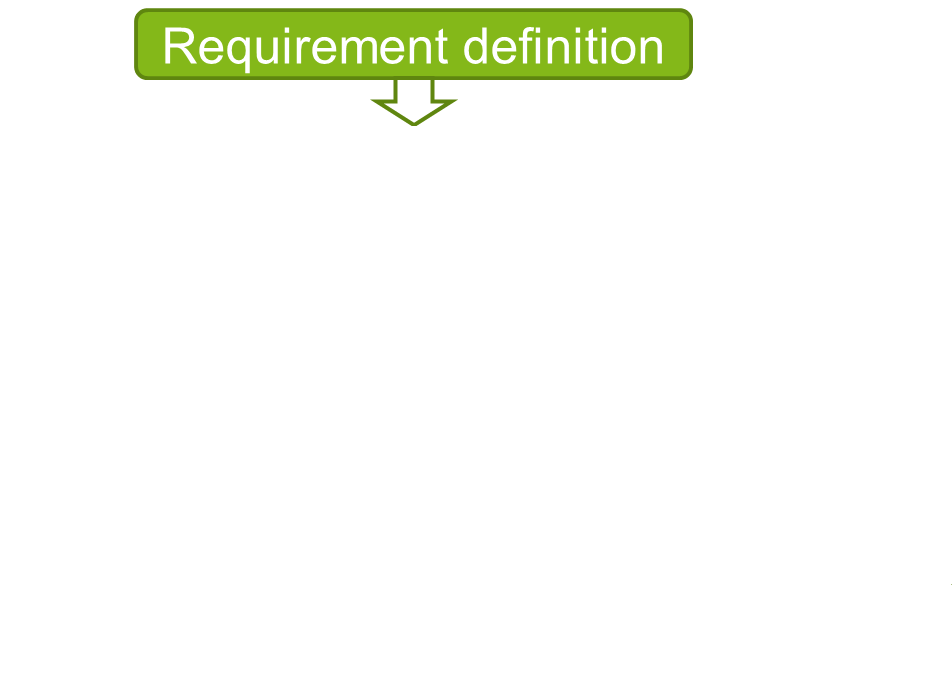
\includegraphics[scale=0.2]{Images/project_schedule_1.png}}{A picture of the first part of a typical software project schedule. It contains the point Requirement specifications.}
			\end{figure}
		\end{frame}
		
		\begin{frame}
			\frametitle{Requirements}
			\begin{itemize}[<+->]
				\item Simple design\\
				$\rightarrow$ High usability
				\item High contrast\\
				$\rightarrow$ Good for visually impaired persons
				\item No distractions\\
				$\rightarrow$ High usability again
				\item Foreseeable behaviour\\
				$\rightarrow$ No confusion
				\item Confirmations\\
				$\rightarrow$ No accidental deletions
				\item Keyboard accessible\\
				$\rightarrow$ For persons dependant on the keyboard
			\end{itemize}
		\end{frame}
	
		\subsection{Software Design}
			\begin{frame}
				\frametitle{Software Design}
				\begin{figure}
					\centering
					\pdftooltip{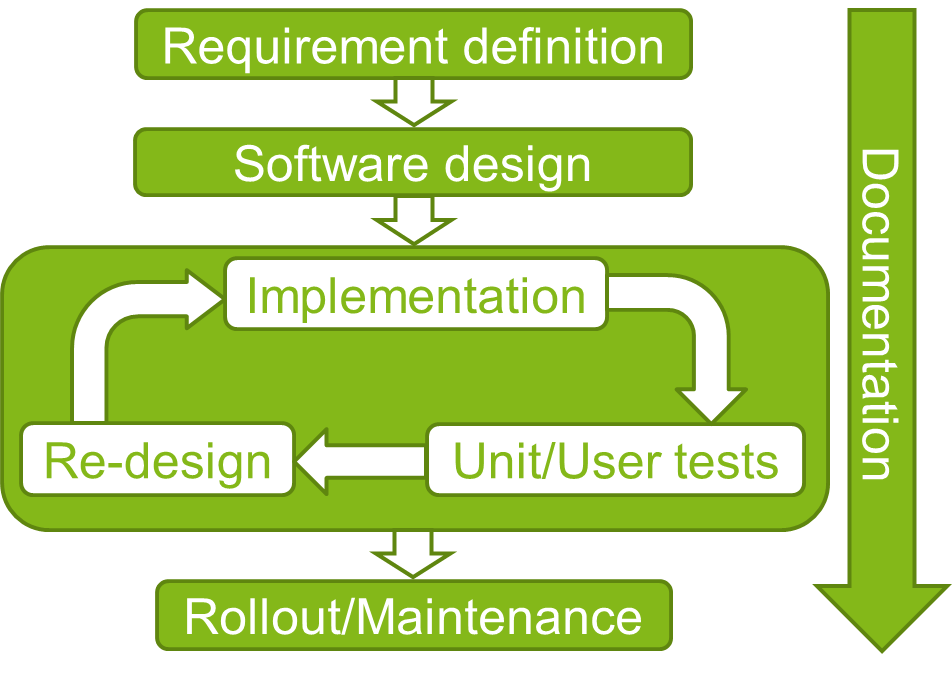
\includegraphics[scale=0.25]{Images/project_schedule_2.png}}{A picture of the first part of a typical software project schedule. It contains the points Requirement specifications and Software design.}
				\end{figure}
			\end{frame}
			
		\subsection{Model}
			\begin{frame}
				\frametitle{Model}
				\begin{itemize}
					\item SQLite Database
					\item Alembic database migration
					\item SQLAlchemy
				\end{itemize}
			\end{frame}
			
		\subsection{View}
			\begin{frame}
				\frametitle{The Kivy Framework}
				\begin{itemize}
					\item Cross platform
					\item Under MIT license
					\item GPU Accelerated
				\end{itemize}
				
				\begin{figure}
					\centering				
					\pdftooltip{
\includegraphics[scale=0.3]{Images/kivy_logo.png}}{The kivy logo.}
					\caption{http://www.kivy.org/ - 02.July, 2014}
				\end{figure}
			\end{frame}
			
			\begin{frame}
				\frametitle{Kivy example}
				\begin{figure}
				\centering
				\pdftooltip{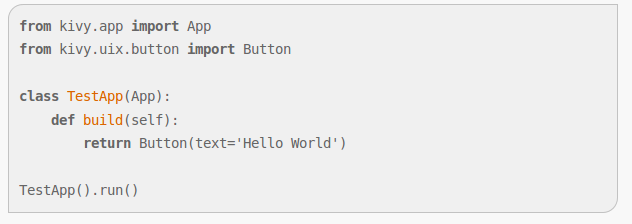
\includegraphics[scale=0.3]{Images/kivy_helloworld_code.png}}{A short kivy code example showing 6 lines of codes.}
				\pdftooltip{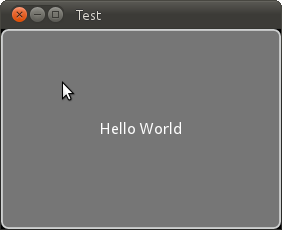
\includegraphics[scale=0.3]{Images/kivy_helloworld_result.png}}{The output of the shown code, which is a functioning GUI.}
				\end{figure}
			\end{frame}
			
		\subsection{Controller}
			\begin{frame}
				\frametitle{Controller}
				Connecting Model and View.\\
				Get emails from server.\\
				The usual logic.
			\end{frame}
			
	\section{Software Development}
	
		\begin{frame}
			\frametitle{Software Development}
			\begin{figure}
				\centering
				\pdftooltip{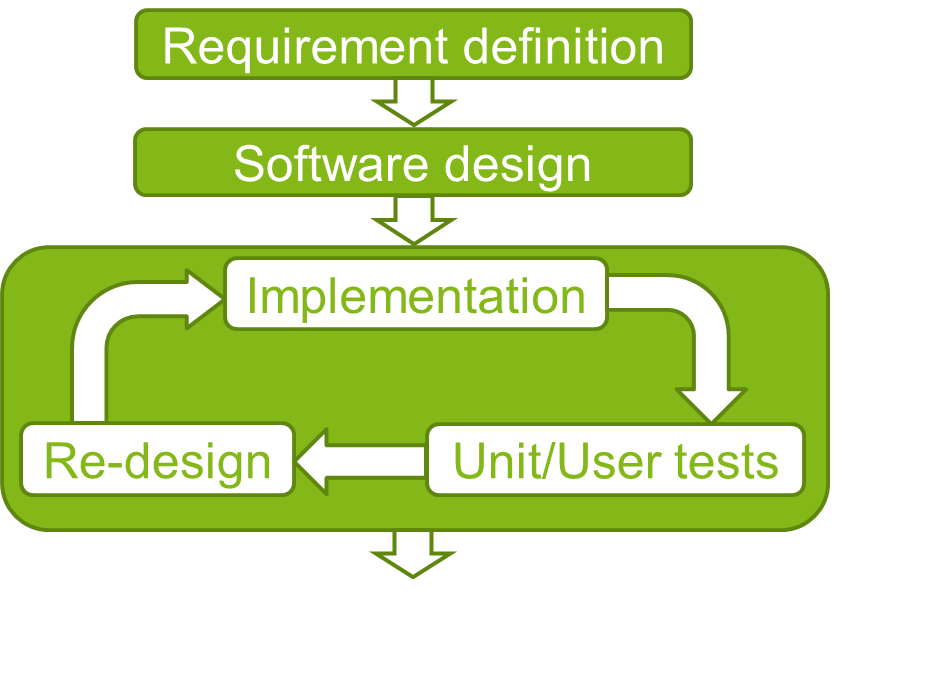
\includegraphics[scale=0.25]{Images/project_schedule_3.png}}{A picture of the first part of a typical software project schedule. It contains the points Requirement specifications, Software design and the Development phase, containing Implementation, Tests and Re-design.}
			\end{figure}
		\end{frame}
		
		\subsection{Implementation}
		
			\begin{frame}
				\frametitle{Implementation}
				\begin{center}
					Business as usual
				\end{center}
			\end{frame}
		
		\subsection{Test routine}
		
			\begin{frame}
				\frametitle{Preparations}
				Aims:
				\begin{itemize}
					\item Test usability
					\item Get feedback on design
					\item (Finding bugs)
				\end{itemize}
			\end{frame}
			
			\begin{frame}
				\frametitle{The script}
				Test the following functions:
				\begin{enumerate}
					\item Create email account
					\item Address book
					\begin{enumerate}
						\item Add contact
						\item Delete contact
						\item Send email to contact
					\end{enumerate}
					\item Email
					\begin{enumerate}
						\item Read email
						\item Write email
						\item Answer email
						\item Delete email
					\end{enumerate}
				\end{enumerate}
			\end{frame}
			
			\begin{frame}
				\frametitle{Test persons}
				\begin{itemize}
					\item 5 persons
					\item Age: 20 to 22
					\item Only private contact with digital media
					\item Contact via Bethel
				\end{itemize}
			\end{frame}
			
			\begin{frame}
				\frametitle{Testing}
				\begin{figure}
					\centering
					\pdftooltip{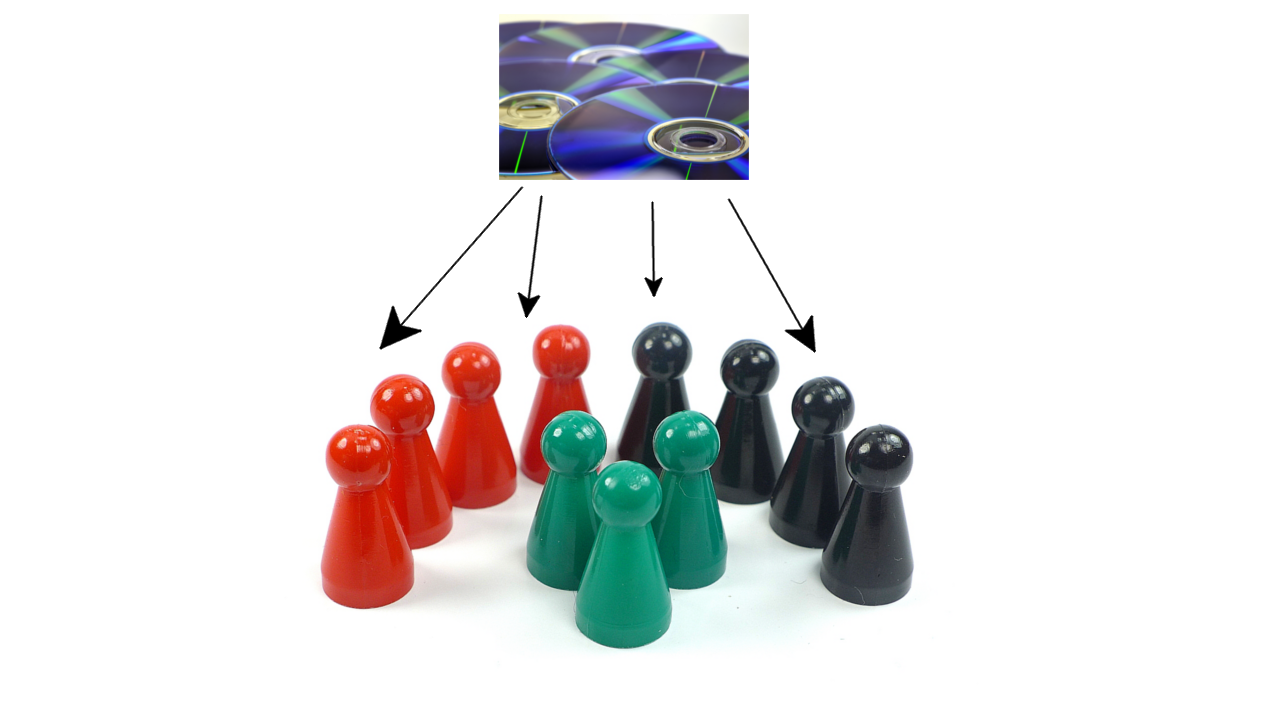
\includegraphics[scale=0.5]{Images/test_distribution.png}}{A picture of a couple of CDs being distributed to toy figures.}
					\caption{www.clearlens-images.de  / pixelio.de, U.Weinreich  / pixelio.de}
				\end{figure}
			\end{frame}
			
			\begin{frame}
				\frametitle{Test routine}
				\begin{itemize}
					\item Live tests with developers
					\item Open discussion
					\item Final and open feedback
				\end{itemize}
			\end{frame}
			
			\begin{frame}
				\frametitle{Test results}
				Results of this routine:
				\begin{enumerate}
					\item Design
					\begin{itemize}
						\item Fancier colours
						\item Smaller symbols
					\end{itemize}
					\item Behaviour
					\begin{itemize}
						\item Buttons not fully intuitive
					\end{itemize}
					\item Demanded Features
					\begin{itemize}
						\item Photos for contacts
						\item Outbox
					\end{itemize}
					\item Technical level
					\begin{itemize}
						\item Email input not reset
						%\item Phantom contacts
					\end{itemize}
				\end{enumerate}
			\end{frame}
			
		
			
%		\subsection{The Software}
%			\begin{frame}
%				\frametitle{GUI}
%				\begin{figure}
%					\centering
%					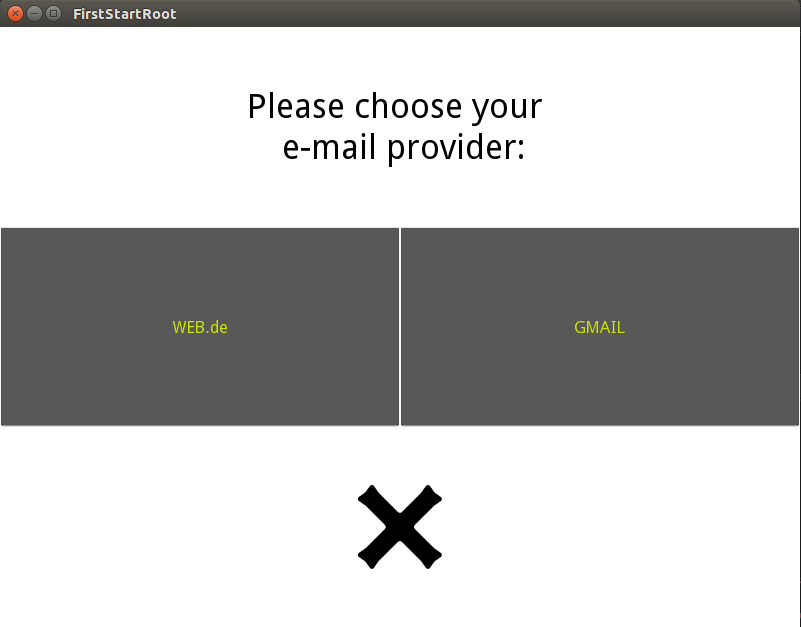
\includegraphics[scale=0.2]{Images/firstStartRoot.png}
%				\end{figure}
%		    	\end{frame}
%		
%			\begin{frame}
%				\frametitle{GUI}
%				\begin{figure}
%					\centering
%					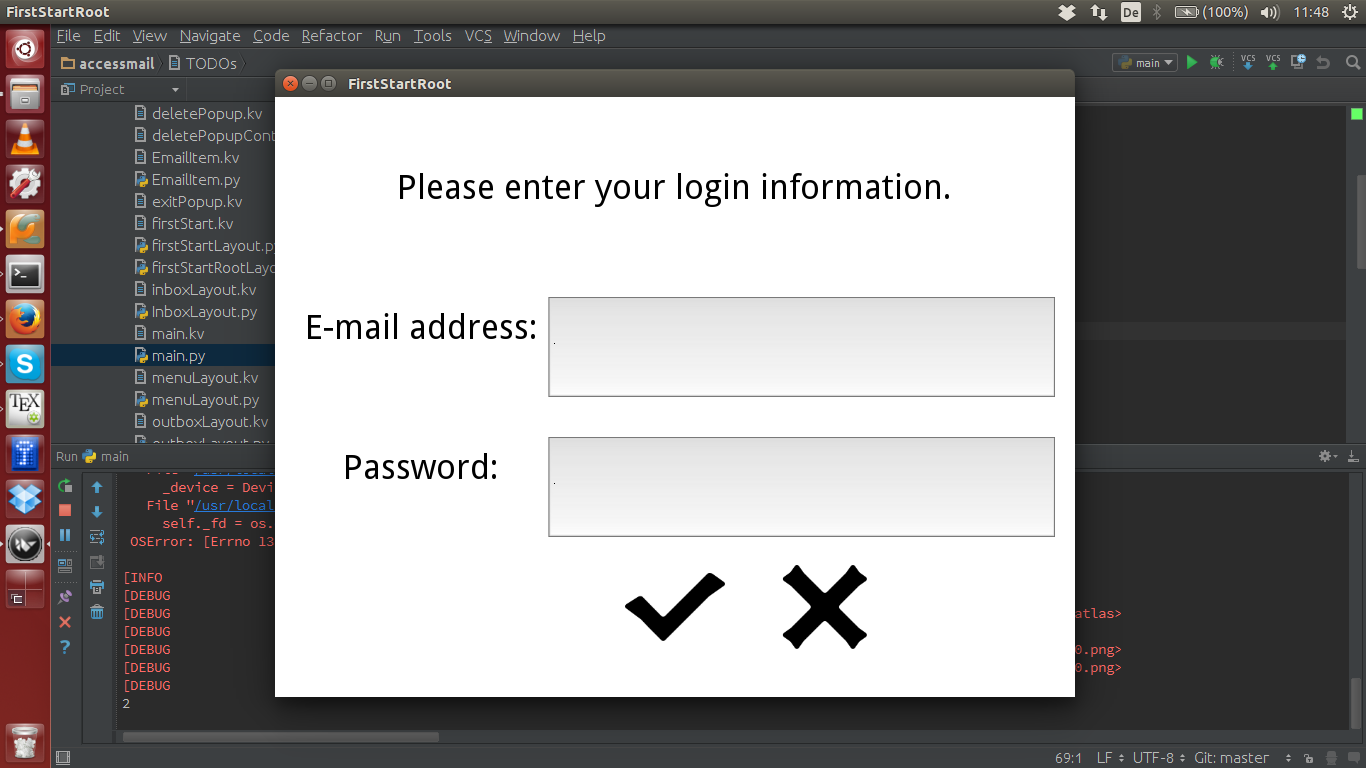
\includegraphics[scale=0.2]{Images/firstStartCredentials.png}
%				\end{figure}
%		    	\end{frame}
%			
%			\begin{frame}
%				\frametitle{GUI}
%				\begin{figure}
%					\centering
%					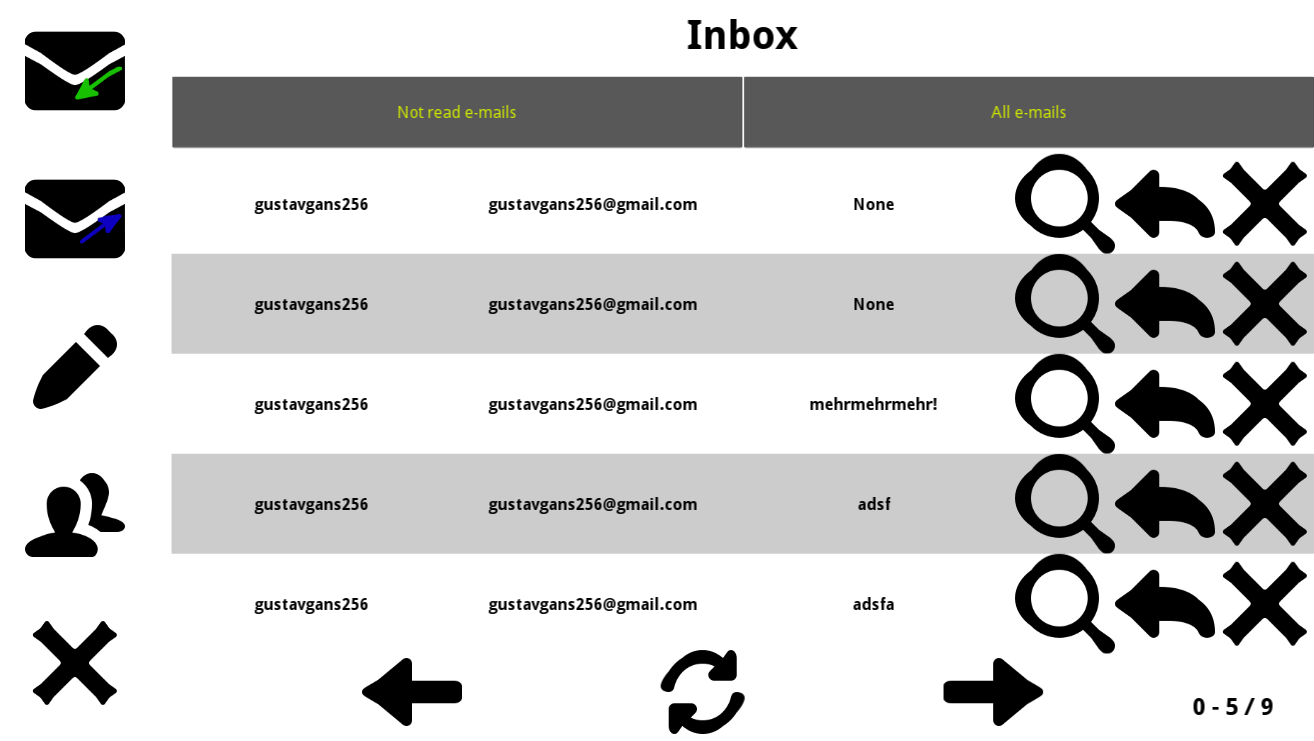
\includegraphics[scale=0.2]{Images/Inbox.png}
%				\end{figure}
%		    	\end{frame}
%			
%			\begin{frame}
%				\frametitle{GUI}
%				\begin{figure}
%					\centering
%					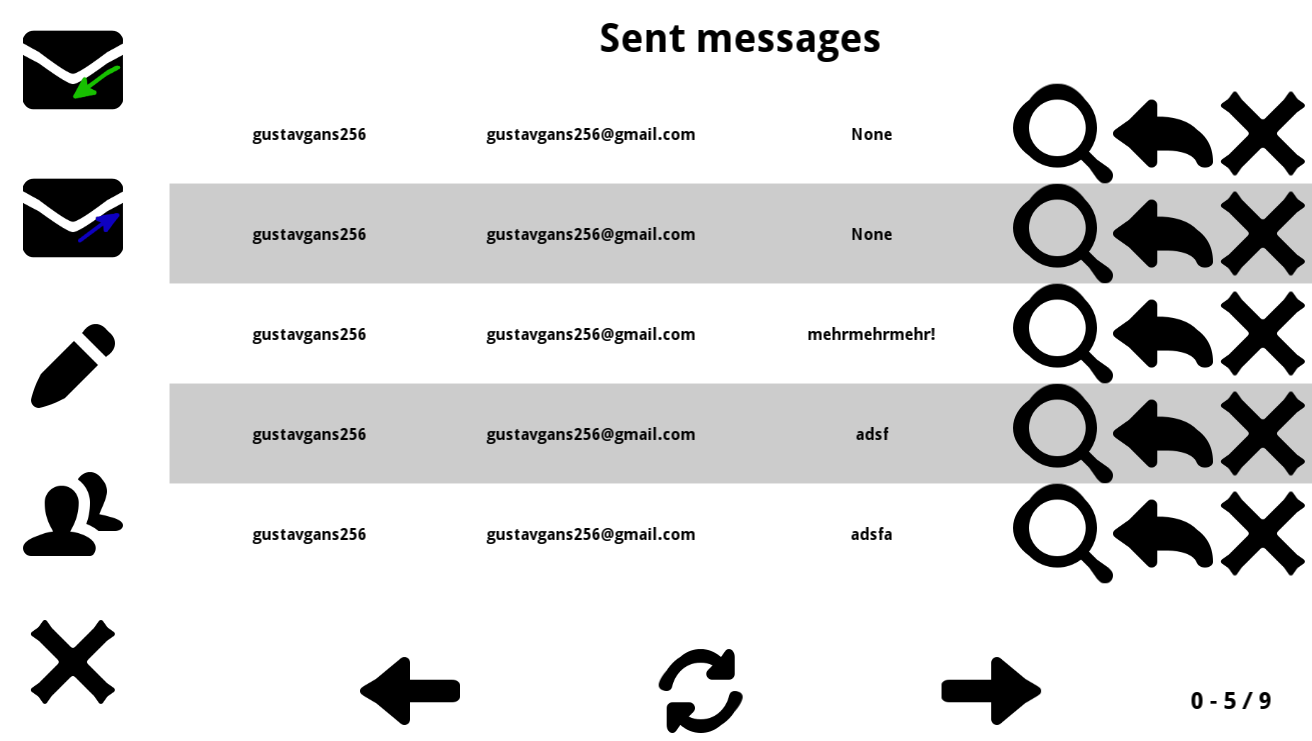
\includegraphics[scale=0.2]{Images/Outbox.png}
%				\end{figure}
%		    	\end{frame}
%		    	
%		    	\begin{frame}
%				\frametitle{GUI}
%				\begin{figure}
%					\centering
%					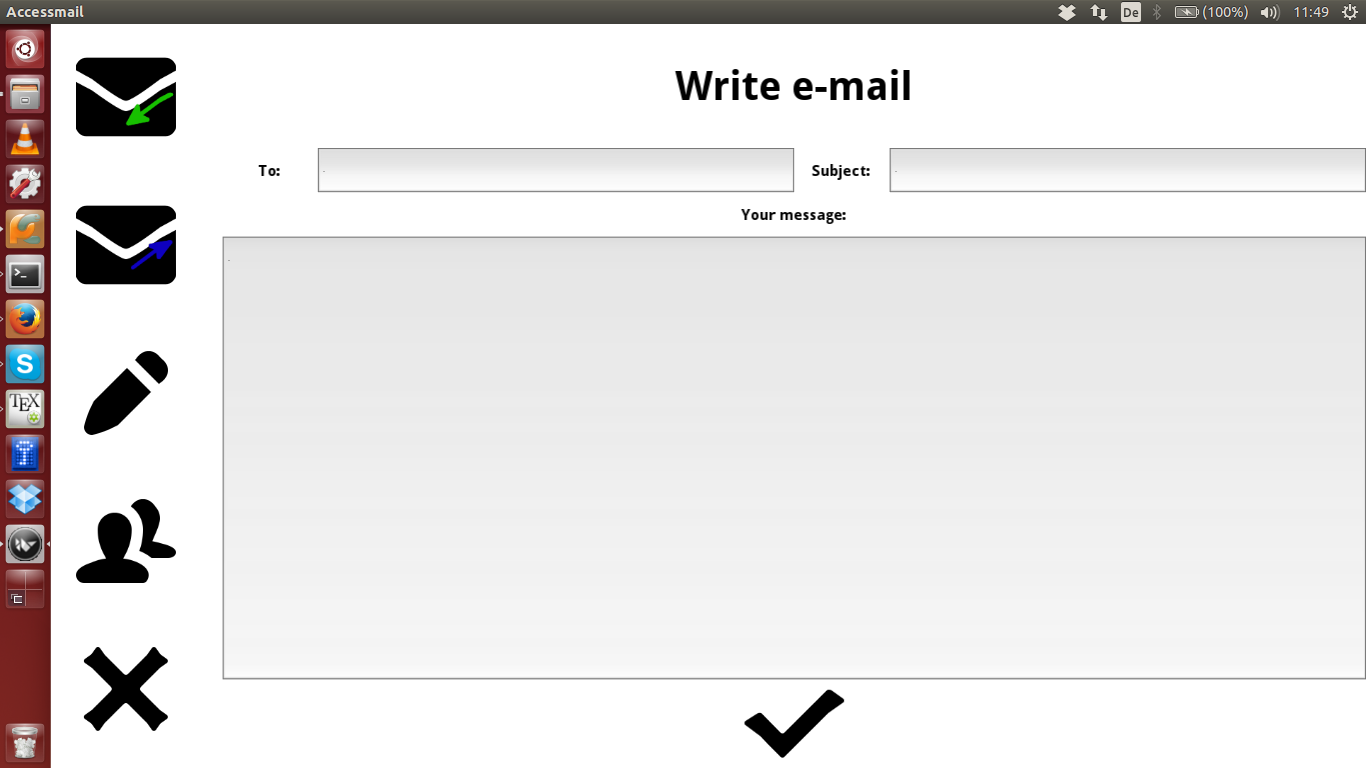
\includegraphics[scale=0.2]{Images/Write_blank.png}
%				\end{figure}
%		    	\end{frame}
%		    	
%		    	\begin{frame}
%				\frametitle{GUI}
%				\begin{figure}
%					\centering
%					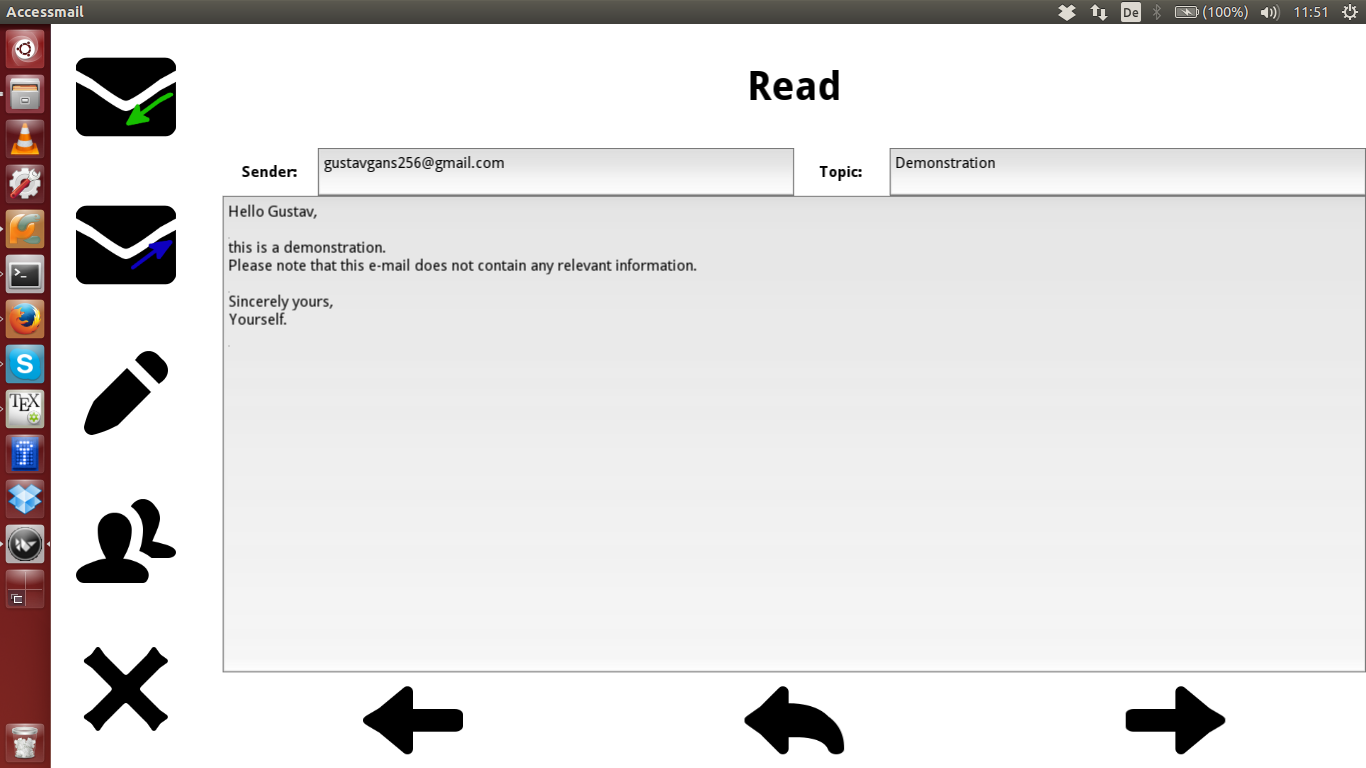
\includegraphics[scale=0.2]{Images/Read.png}
%				\end{figure}
%		    	\end{frame}
%		    	
%		    	\begin{frame}
%				\frametitle{GUI}
%				\begin{figure}
%					\centering
%					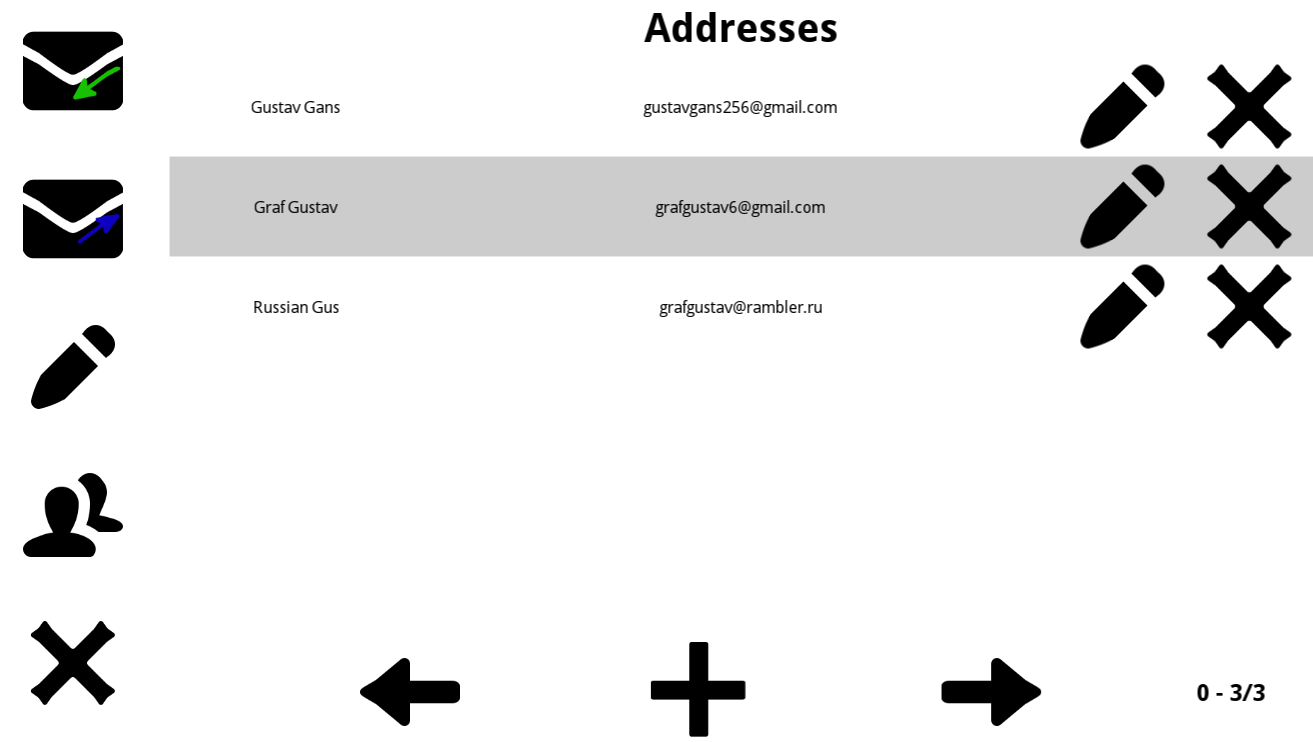
\includegraphics[scale=0.2]{Images/Addresses.png}
%				\end{figure}
%		    	\end{frame}
%		    	
%		    	\begin{frame}
%				\frametitle{GUI}
%				\begin{figure}
%					\centering
%					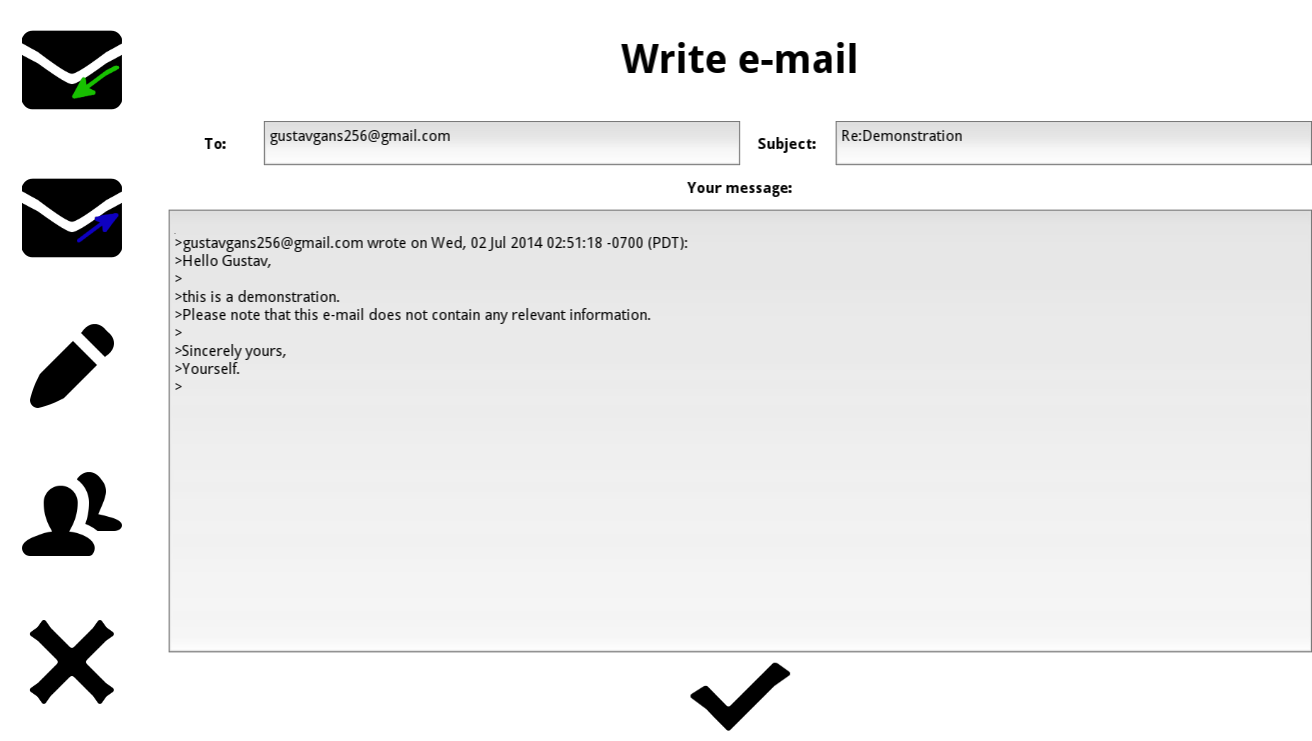
\includegraphics[scale=0.2]{Images/Answer.png}
%				\end{figure}
%		    	\end{frame}
%			\begin{frame}
%				\frametitle{Techniques}
%				
%		    	\end{frame}
		    	
	
	\section{Conclusion}
	
		\subsection{The software}
		
			\begin{frame}
				\frametitle{Software Design}
				\begin{figure}
					\centering
					\pdftooltip{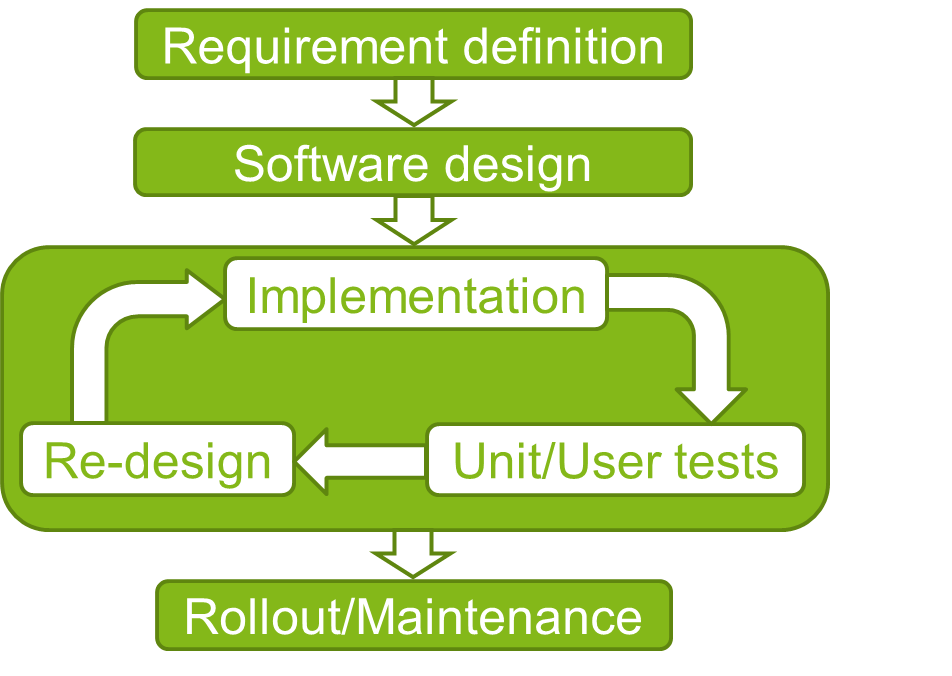
\includegraphics[scale=0.25]{Images/project_schedule_4.png}}{A picture of the first part of a typical software project schedule. It contains the points Requirement specifications, Software design and the Development phase, containing Implementation, Tests and Re-design. The last point is the Rollout/Maintenance.}
				\end{figure}
			\end{frame}
			
			\begin{frame}
				\begin{center}
					Let us have a look at the software!
				\end{center}
			\end{frame}
			
		\subsection{Conclusions}
			
			\begin{frame}
				\frametitle{Conclusions}
				\begin{center}
					\begin{tabular}{ l | c | r }
						\hline
						\textbf{Successful} & \textbf{Planned} & \textbf{Testing results}\\
						Simple design & Keyboard support & Contact photos\\
						High contrast & More provider & Updated design\\
						No distractions & Attachments & Introduction to email\\
						Foreseeable behaviour & \hfill & \hfill \\
						\hline
					\end{tabular}
				\end{center}
			\end{frame}
			
			\begin{frame}
				\frametitle{We are open to questions now}
				\begin{figure}
					\centering
					\pdftooltip{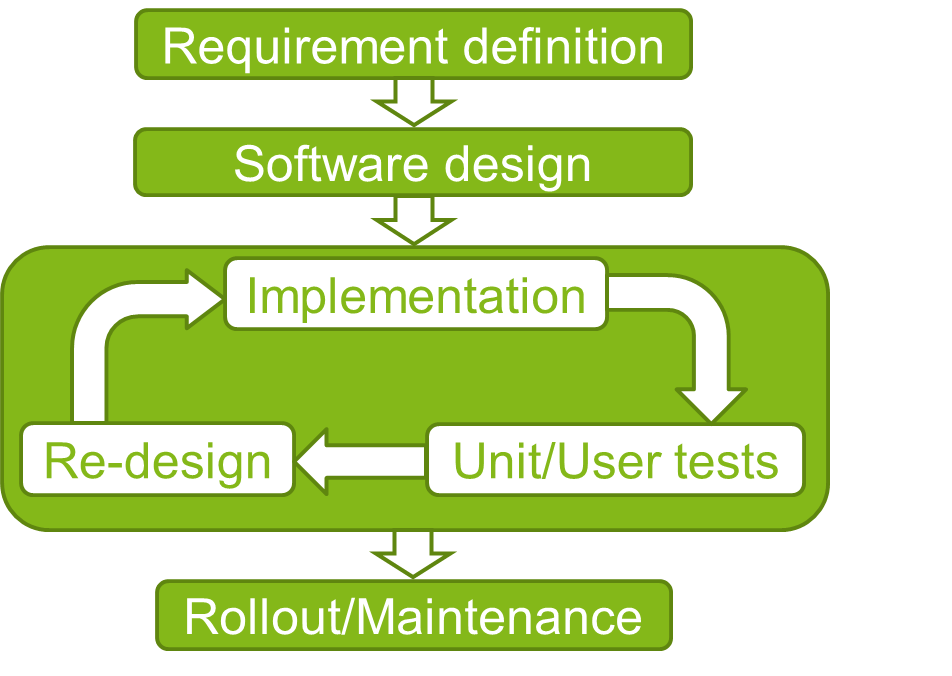
\includegraphics[scale=0.25]{Images/project_schedule_4.png}}{A picture of the first part of a typical software project schedule. It contains the points Requirement specifications, Software design and the Development phase, containing Implementation, Tests and Re-design. The last point is the Rollout/Maintenance.}
				\end{figure}
			\end{frame}

\end{document}
